% #####################################################################
% #####################################################################
% ##                                                                 ##
% ##                             Lizenz:                             ##
% ##                         CC BY-NC-SA 3.0                         ##
% ##      http://creativecommons.org/licenses/by-nc-sa/3.0/de/       ##
% ##                                                                 ##
% #####################################################################
% ##   Diese Datei kann beliebig verändert werden, solange darauf    ##
% ##     hingewiesen wird, dass dieses Dokument ursprünglich von     ##
% ##                                                                 ##
% ##                        www.ei-studium.de                        ##
% ##                                                                 ##
% ##                             stammt.                             ##
% ## Dies gilt insbesondere auch für alle daraus erstellten Dateien. ##
% ##    Des Weiteren muss die Weitergabe dieser Dateien unter der    ##
% ##                    gleichen Lizenz erfolgen.                    ##
% #####################################################################
% #####################################################################
\documentclass[a4paper,twocolumn,10pt]{article}
\usepackage[utf8]{inputenc}
\usepackage[ngerman]{babel}
\usepackage[top=2.0cm,bottom=1.5cm,left=1.0cm,right=1.0cm]{geometry}
\usepackage{enumitem}
\usepackage{graphicx}
\usepackage{amsfonts}
\usepackage{amsmath}
\usepackage{sectsty}
\usepackage{colortbl}
\usepackage{cancel}
\usepackage{listings}
\usepackage{color}
\usepackage{amsmath}
\usepackage{trfsigns}
\usepackage{extarrows}
\usepackage{epstopdf}
\usepackage{fancyhdr}
\usepackage[pdfborder={0 0 0}]{hyperref}

\setlist{itemsep=.01mm}
\setenumerate{label=\emph{\arabic*})}
\setlength{\columnsep}{1cm}
\parindent 0mm

\partfont{\Large}
\sectionfont{\large \sc\bf}
\subsectionfont{\normalsize}
\subsubsectionfont{\small\textit}

\pagestyle{fancy}
\lhead[\leftmark]{FS Werkstoffe der Elektrotechnik}
\chead[\leftmark]{\url{http://www.ei-studium.de}}
\rhead[\leftmark]{Erstelldatum: \today}
\lfoot[\leftmark]{Keine Garantie auf Vollständigkeit und Richtigkeit!}
\cfoot[\leftmark]{}
\rfoot[\leftmark]{\thepage}
\renewcommand{\headrulewidth}{0.5pt}
\renewcommand{\footrulewidth}{0.5pt}

\newcommand{\sollsein}{\stackrel{!}{=}}
\newcommand*\kreis[1]{\unitlength1ex\begin{picture}(2.5,2.5)%
\put(0.75,0.75){\circle{3}}\put(0.7,0.7){\makebox(0,0){#1}}\end{picture}}

\begin{document}
{\small \tableofcontents}
\newpage

\part{Werkstoffe der Elektrotechnik}

\section{Aufbau der Materie}

\subsection{Quanten und Wellen}
\begin{equation*}
\begin{split}
\text{Wellenlänge: }\lambda&=\frac{c}{f}=\frac{h}{p}=\frac{h}{mv} \\
\text{Energie: }E&=mc^2=\hbar\omega=hf=\frac{hc}{\lambda} \\
\text{Impuls: }p&=mv=\hbar k=\frac{\hbar \omega}{c}=\frac{h}{\lambda} \\
\text{Wellenzahl: }k&=\frac{2\pi}{\lambda} \\
\text{Phasengeschwindigkeit: }v_{Ph}&=\frac{\omega}{k}=\frac{\hbar k}{2m}=\frac{v_{Teilchen}}{2}\\
\text{Gruppengeschwindigkeit: }v_{gr}&=\frac{\partial\omega}{\partial k}=\frac{\hbar k}{m}=\frac{p}{m}\\
\text{Dispersionsrelation: }E&=\omega\hbar =\frac{\hbar^2k^2}{2m}
\end{split}
\end{equation*}

\subsubsection{Schrödingergleichung}
\textbf{Herleitung:}\\
Ausgehend von der Dispersionsrelation:
\begin{equation*}
\begin{split}
&\omega\laplace -j\frac{\partial}{\partial t}\\
&k\laplace j\nabla
\end{split}
\end{equation*}
\textbf{Allgemeine Schrödingergleichung:}
\begin{equation*}
-j\hbar\frac{\partial}{\partial t}\Psi (\overrightarrow{r},t)=-\frac{\hbar^2}{2m^*}\Delta\Psi(\overrightarrow{r},t)+V(\overrightarrow{r},t)\Psi(\overrightarrow{r},t)
\end{equation*}
\textbf{Zeitunabhängige Schrödingergleichung:}\\
Durch den Separationsansatz $\Psi(\overrightarrow{r},t)=\Psi(\overrightarrow{r})\Phi(t)$ lässt sich die Zeitabhängigkeit abtrennen:
\begin{equation*}
-\frac{\hbar^2}{2m^*}\Delta\Psi(\overrightarrow{r})+V(\overrightarrow{r})\Psi(\overrightarrow{r})=E\Psi(\overrightarrow{r})
\end{equation*}

\subsubsection{1-dimensinaler Potentialtopf}
\textbf{Ansatz für DGL:}
\begin{equation*}
\Psi(x)=Ae^{jkx}+Be^{-jkx}
\end{equation*}
bzw.
\begin{equation*}
\Psi(x)=Asin(kx)+Bcos(kx)
\end{equation*}\\
Für den jeweiligen Bereich mit dem Potential $V$ gilt:
\begin{equation*}
k=\frac{\sqrt{2m^*(E-V)}}{\hbar}
\end{equation*}
Im Falle von unendlich hohen Barrieren und der Breite $a$ gilt:
\begin{equation*}
\begin{split}
\Psi_n(x)&=\sqrt{\frac{2}{a}}sin\left(\frac{n\pi}{a}x\right) \\
E&=\frac{\hbar^2\pi^2}{2m^*a^2}n^2=\frac{\hbar^2}{2m^*}k^2 \\
\text{mit }k&=\frac{n\pi}{a}
\end{split}
\end{equation*}
\textbf{Randbedingungen:}\\
Für die Wellenfunktion $\Psi(x)$ gelten folgende Randbedingungen:
\begin{enumerate}[label=$\bullet$]
\item $\Psi(x)$ ist stetig (ohne Sprung)
\item $\Psi(x)$ ist differenzierbar
\item $\int\limits_{-\infty}^{\infty}|\Psi(x)|^2dx=\int\limits_{-\infty}^{\infty}\Psi^*(x)\Psi(x)dx=1$
\end{enumerate}

\subsubsection{3-dimensionaler Potentialtopf}
Die Lösung erfolgt wie beim 1-dimensionalen Potentialtopf durch den Separationsansatz
\begin{equation*}
\Psi(x,y,z)=\Psi(x)\Psi(y)\Psi(z)
\end{equation*}
Im Falle eines Würfels mit Kantenlänge $a$ und unendlich hohen Barrieren gilt:
\begin{equation*}
\begin{split}
\Psi_{nml}(x,y,z)&=\sqrt{\frac{8}{a^3}}sin\left(\frac{n\pi}{a}x\right)sin\left(\frac{m\pi}{a}y\right)sin\left(\frac{l\pi}{a}z\right)\\
E&=\frac{\hbar^2\pi^2}{2m^*a^2}(n^2+m^2+l^2) \\
E&=\frac{\hbar^2}{2m^*}(k_x^2+k_y^2+k_z^2)
\end{split}
\end{equation*}

\subsubsection{Sonstiges}
\textbf{Teilchenstromdichte:}
\begin{equation*}
j=(\Psi^*\Psi)v_{gr}=(\Psi^*\Psi)\frac{\hbar k}{m_0}
\end{equation*}
Reflexionskoeffizient: $\frac{j_R}{j_0}$\\
Transmissionskoeffizient: $\frac{j_T}{j_0}$

\subsection{Wasserstoffatom}
$a$: Bohrscher Atomradius, $R_H$: Rydbergkonstante\\
$\lambda$: emittierte bzw. absorbierte Wellenlänge\\\\
Für die Energieniveaus eines $H$-Atoms gilt:
\begin{equation*}
\begin{split}
E_n&=-\frac{\hbar^2}{2m_0}\left(\frac{1}{na}\right)^2=-\underbrace{\frac{m_0e^4}{2(4\pi\epsilon_0\hbar)^2}}_{2,18\cdot 10^{-18}J}\frac{1}{n^2}\\
\lambda&=\frac{1}{R_H\left|\frac{1}{n^2}-\frac{1}{m^2}\right|};\;\;\;\;n,m\in\mathbb{N}
\end{split}
\end{equation*}

\subsection{Aufbau des Periodensystems}
$\rightarrow$ siehe Skript S. 24

\subsubsection{Quantenzahlen}
\textbf{Hauptquantenzahl:}\\
$\hat{=}$ Energieeigenwerte\\
$n=1,2,...$ ($\hat{=} K,L,...$-Schale) \\\\
\textbf{Nebenquantenzahl:}\\
$\hat{=}$ Orbitalgestalt\\
$l=0,...,n-1$ ($\hat{=} s,p,d,f$-Zustände)\\\\
\textbf{Magnetische Quantenzahl:}\\
$\hat{=}$ Orientierung der Orbitale\\
$m=-l,-l+1,...,l-1,l\;\;(\widehat{=}L)$\\\\
\textbf{Spinquantenzahl:}\\
$s=\pm \frac{1}{2}$\\\\
\textbf{Entartungsgrad:}\\
Anzahl der Kombinationen der Quantenzahlen mit gleicher Energie.\\
$\Rightarrow 2n^2$\\
\begin{center}
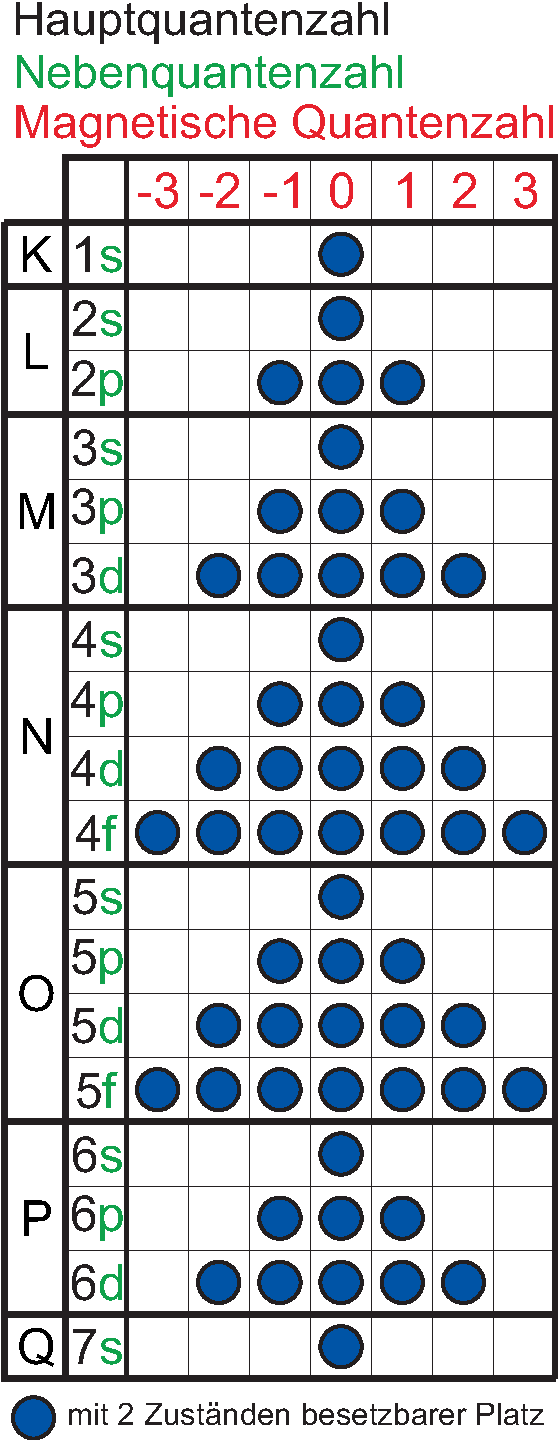
\includegraphics[width=0.6\columnwidth]{Grafiken/Quantenzahlen}
\end{center}

\subsubsection{Pauli-Prinzip}
Alle Elektronen unterscheiden sich in mindestens einer Quantenzahl.

\subsubsection{Hundsche Regeln}
\begin{enumerate}
\item Schale wird so aufgefüllt, dass
\begin{equation*}
|S|=\left|\sum s_i\right|\text{ mit }s=\pm \frac{1}{2}
\end{equation*}
maximal wird.
\item Quantenzahl $|L|$ maximal.
\item
\begin{enumerate}[label=$\bullet$]
\item Schale weniger als halbvoll
\begin{enumerate}[label=-]
\item Bahndrehimpuls und Spin antiparallel
\item Gesamtdrehimpuls $|J|=||L|-|S||$
\end{enumerate}
\item Schale mehr als halbvoll
\begin{enumerate}[label=-]
\item Bahndrehimpuls und Spin parallel
\item Gesamtdrehimpuls $|J|=|L|+|S|$
\end{enumerate}
\end{enumerate}
\end{enumerate}
Volle Schalen liefern keinen Beitrag zu $S,L$ und $J$!
\begin{center}
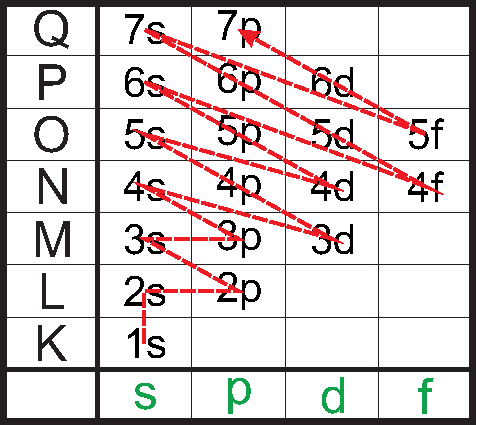
\includegraphics[width=0.6\columnwidth]{Grafiken/Hundsche_Regeln}
\end{center}

\subsection{Bindungstypen}

\subsubsection{Ionische Bindung}
$\hat{=}$ Bindung durch Elektronenaustausch\\\\
\underline{Voraussetzung:}
\begin{enumerate}[label=$\bullet$]
\item Unterschiedliche, leicht zu ionisierende Atome
\item Differenz der Elektronegativität i.d.R. $\Delta E >1,7$
\end{enumerate}
Die Ionisierung läuft prinzipiell in 3 Schritten ab:
\begin{enumerate}
\item Ionisierung des Kations (Energiezufuhr)
\item Ionisierung des Anions (Energieabgabe)
\item Molekülbildung (Energieabgabe)
\end{enumerate}
Die elektrische Bindungsenergie, die bei der Molekülbildung frei wird, berechnet sich wie folgt:
\begin{equation*}
E_{el}=\int\limits_{\infty}^{r_0}-\frac{q_1q_2}{4\pi\epsilon_0r^2}dr=\frac{q_1q_2}{4\pi\epsilon_0r_0}
\end{equation*}
wobei $r_0$ der Abstand ist und $q_1,q_2$ die Ladungen der Ionen darstellen.

\subsubsection{Kovalente Bindung}
$\hat{=}$ Bindung durch gemeinsame Elektronen\\\\
\underline{Voraussetzung:}
\begin{enumerate}[label=$\bullet$]
\item Differenz der Elektronegativität i.d.R. $\Delta E < 1,7$
\end{enumerate}

\subsubsection{Metallische Bindung}
= Sonderfall der kovalenten Bindung, bei der die Valenzelektronen nicht lokalisiert sind.

\subsection{Aggregatzustände der Materie}

\subsubsection{Gase}
$p$: Druck, $V$: Volumen, $T$: Temperatur, $\rho$: Dichte\\
$n_A$: Anzahl Atome, $k_B$: Boltzmannkonstante\\
$n_{mol}$: Stoffmenge, $R$: Gaskonstante, $N$: Teilchendichte\\
$N_A$: Avogadro-Konstante, $A_r$: Relative Atommasse\\
$M$: Molare Masse, $u$: Atomare Masseneinheit\\
\begin{equation*}
\begin{split}
\frac{pV}{T}&=n_{mol}R=n_Ak_B=\frac{n_AR}{N_A};\;\;\;\;[n_{mol}R]=\frac{J}{K}\text{ (ideales Gas)}\\
M&=A_r\cdot 10^{-3}\frac{kg}{mol};\;\;\;\;[A_r]=1\\
n_{mol}&=\frac{n_A}{N_A}=\frac{m}{M}\\
R&=N_Ak_B\\
p&=\frac{1}{3}Nm\overline{v^2}=Nk_BT\\
N&=\frac{n_A}{V}=\frac{n_{mol}N_A}{V}=\frac{\rho N_A}{M}=\frac{p}{k_BT}\\
\rho &=\frac{NM}{N_A}=\frac{n_AA_ru}{V}=\frac{m}{V}\\
E_{kin}&=\frac{1}{2}m\overline{v^2}=\frac{f}{2}k_BT
\end{split}
\end{equation*}
mit $f$: Anzahl der Freiheitsgrade ($=3$ für einatomige Gase)

\subsection{Kristallstrukturen}
$KZ$: Koordinationszahl (Zahl der nächsten Nachbarn)\\
$n_{EZ}$: Anzahl der Atome pro Einheitszelle (EZ)\\
$r$: Atomradius\\
\begin{center}
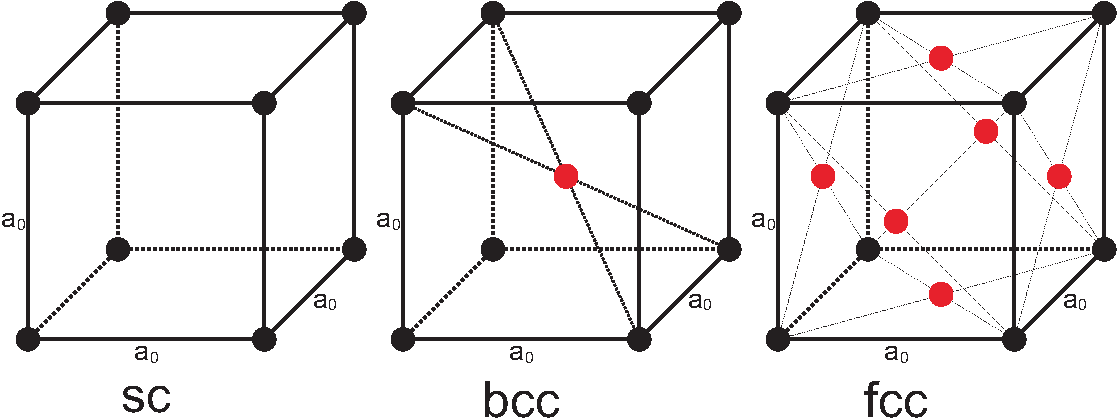
\includegraphics[width=0.9\columnwidth]{Grafiken/Kristallstrukturen}
\end{center}
\textbf{Packungsdichte:}
\begin{equation*}
P=\frac{\text{Volumen (Atome)}}{\text{Volumen (EZ)}}=\frac{n_{EZ}\frac{4}{3}\pi r^3}{V_{EZ}}=\frac{4n_{EZ}\pi r^3}{3a_0^3}
\end{equation*}
\textbf{Achtung:}\\
Für die Berechnung von $n_{EZ}$ müssen Atome, die von angrenzenden Zellen auch verwendet werden, dementsprechend gewichtet werden!

\subsubsection{Primitiv kubisch (sc)}
(=simple cubic)
\begin{equation*}
\begin{split}
n_{EZ}&=1\\
r&=\frac{1}{2}a_0\\
KZ&=6\\
P&=\frac{1}{6}\pi\approx 0,52
\end{split}
\end{equation*}

\subsubsection{Kubisch raumzentriert (bcc)}
(=body centered cubic)
\begin{equation*}
\begin{split}
n_{EZ}&=2\\
r&=\frac{\sqrt{3}}{4}a_0\\
KZ&=8\\
P&=\frac{\sqrt{3}}{8}\pi\approx 0,68
\end{split}
\end{equation*}

\subsubsection{Kubisch flächenzentriert (fcc)}
(=face centered cubic)
\begin{equation*}
\begin{split}
n_{EZ}&=4\\
r&=\frac{\sqrt{2}}{4}a_0\\
KZ&=12\\
P&=\frac{\sqrt{2}}{6}\pi\approx 0,74
\end{split}
\end{equation*}

\subsection{Metalle und Legierungen}

\subsubsection{Mischkristallbildung durch Leerstellendiffusion}
$S$: Teilchenstromdichte, $D$: Diffusionskoeffizient\\
$N$: Teilchenkonzentration, $x_D$: Mittlere Eindringtiefe\\
$E_A$: Aktivierungsenergie für Leerstellendiffusion
\begin{equation*}
\begin{split}
S&=-D\frac{\partial N}{\partial x}\\
D&=D_0e^{-\frac{E_A}{k_BT}};\;\;\;\;\;[D]=\frac{cm^2}{s}\\
x_D&=\sqrt{Dt}
\end{split}
\end{equation*}

\section{Mechanische Eigenschaften der Festkörper}
$\rho$: Dichte, $\epsilon$: Dehnung, $\sigma$: Mech. Spannung (= Druck)\\
$E$: Elastizitätsmodul, $V$: Volumen, $P$: Packungsdichte\\
$r$: Atomradius, $a_0$: Gitterkonstante, $m_A$: Atommasse\\
$n_{EZ}$: Anzahl der Atome pro Einheitszelle\\
$\alpha$: Längenausdehnungskoeffizient
\begin{equation*}
\begin{split}
\rho&=\frac{m_AP}{\frac{4}{3}\pi r^3}=\frac{m_An_{EZ}}{a_0^3};\;\;\;\;[\rho]=\frac{kg}{m^3}\\
\epsilon&=\frac{\Delta l}{l}=\alpha\Delta T\\
\sigma&=\frac{F}{A}=\epsilon E=\alpha\Delta TE;\;\;\;\;[\sigma]=\frac{N}{m^2}\\
E&=-\frac{1}{r_0}\left.\frac{dF}{dr}\right|_{r=r_0};\;\;\;\;[E]=\frac{N}{m^2}
\end{split}
\end{equation*}
$V(r)$: Wechselwirkungsenergie, $p$: Druck\\
$K$: Kompressionsmodul; $F(r)$: Kraft (im Gleichgewicht)\\
$\nu$: Poissonsche Zahl
\begin{equation*}
\begin{split}
V(r)&=\underbrace{-\frac{\alpha}{r^n}}_{\text{anziehend}}+\underbrace{\frac{\beta}{r^m}}_{\text{abstoßend}};\;\;\;n<m\\
\text{Für Ionen gilt: }n=1\\
F(r)&=-\frac{dV}{dr}\\
K&=-\frac{p}{\frac{\Delta V}{V}}=\frac{E}{3(1-2\nu)}\\
\end{split}
\end{equation*}
Im Normalfall gilt: $\nu =0,3\Rightarrow K\approx 0,8E$

\section{Thermische Eigenschaften der Festkörper}

\subsection{Spezifische Wärme}
$C$: Wärmekapazität, $c$: Spezifische Wärmekapazität\\
$c_m$: Molwärme, $U$: Innere Energie $T$: Temperatur\\
$n_A$: Anzahl der Atome, $k_B$: Boltzmannkonstante, $m$: Masse\\
$M$: Molare Masse, $R$: Gaskonstante, $T_F$: Fermi-Temperatur\\
$E_F$: Fermi-Energie
\begin{equation*}
\begin{split}
C&=\frac{\partial U}{\partial T}=cm=3n_Ak_B=\frac{3Rm}{M};\;\;\;\;[C]=\frac{J}{K};\;[A_r]=\frac{g}{mol}\\
c&=\frac{C}{m}=\frac{1}{m}\frac{\Delta U}{\Delta T}=\frac{c_m}{M}=\frac{3n_Ak_B}{m}=\frac{3R}{M};\;\;\;\;[c]=\frac{J}{kgK}\\
c_m&=\underbrace{3R}_{Atome}+\underbrace{\frac{6RT}{T_F}}_{Elektronen}=3R\left(1+2\frac{T}{T_F}\right);\;\;\;[c_m]=\frac{J}{molK}\\
&\text{Elektronen-Anteil kann für hohe $T$ vernachlässigt werden!}\\
c_m&=3R=24,9\frac{J}{mol K}\text{ für hohe Temperaturen}\\
T^3&\sim C,c,c_m\text{ für niedrige Temperaturen}\\
T_F&=\frac{E_F}{k_B}\\
R&=k_BN_A\\
U&=3Nk_BT
\end{split}
\end{equation*}

\subsection{Thermische Ausdehnung}
$\Delta l$: Längenausdehnung, $\Delta V$: Volumenausdehnung\\
$\alpha$: Längenausdehnungskoeffizient, $T_S$: Schmelztemperatur\\
$\beta$: Volumenausdehnungskoeffizient
\begin{equation*}
\begin{split}
\Delta l&=\alpha l_0\Delta T\\
\Delta V&=\beta V_0\Delta T\approx 3\alpha V_0\Delta T\\
\beta&\approx 3\alpha\\
\alpha&\sim\frac{1}{T_S}\;\;\;\;\text{(Grüneisen-Regel)}
\end{split}
\end{equation*}

\subsection{Wärmeleitung}
$Q$: Wärmemenge, $A$: Querschnitt, $W$: Wärmestromdichte\\
$I$: Wärmestrom ($\widehat{=}$ Leistung), $\lambda$: Wärmeleitfähigkeit\\
$\frac{\Delta Q}{A}$: Transportierte Wärmemenge, $G$: Wärmeleitwert\\
$v_x$: Geschwindigkeit in x-Richtung, $n$: Teilchendichte
\begin{equation*}
\begin{split}
\nabla T&=\frac{T_a(t)-T_b(t)}{l}\Rightarrow\;\;\kreis{b}\xlongrightarrow{\text{x}} \;\kreis{a}\\
\frac{\Delta Q}{A}&=-\lambda \nabla T\Delta t\\
Q&=CT;\;\;\;\;[Q]=J\\
I&=\dot{Q}=-\lambda A\nabla T=G\Delta T=C_a\dot{T}_a=-C_b\dot{T}_b\\
G&=\lambda\frac{A}{l};\;\;\;\;[G]=\frac{K}{W};\;[\lambda]=\frac{W}{Km}\\
W&=\frac{\dot{Q}}{A}=\frac{\Delta Q}{A\Delta t}=nv_x c\Delta T\\
\end{split}
\end{equation*}
$l_x$: Freie Weglänge zwischen zwei Streuprozessen\\
$C_{Ph}$: Wärmekapazität der Phononen pro Volumeneinheit\\
$\nu$: Schallgeschwindigkeit, $\tau$: Streuzeit\\
\begin{equation*}
\begin{split}
\Delta T&=-\frac{dT}{dx}l_x\\
l&=v\tau\\
\lambda&=\frac{1}{3}lC\sqrt{\overline{v^2}}=\frac{1}{3}C_{Ph}\nu l;\;\;\;\;[\lambda]=\frac{W}{Km}
\end{split}
\end{equation*}
Differentialgleichungen sind mit folgendem Ansatz zu lösen:
\begin{equation*}
T(0,t)=De^{-Et}+F
\end{equation*}

\subsection{Freies Elektronengas / spezifische Wärme der Elektronen}
$D(E)$: Zustandsdichte, $f(E,T)$: Fermiverteilung\\
$n$: Elektronendichte, $E_F$: Fermienergie\\
\begin{equation*}
\begin{split}
D(k)&\sim k^2\\
D(E)&=\frac{1}{V}\frac{dZ}{dE}=\left(\frac{2m}{\hbar^2}\right)^{\frac{3}{2}}\frac{1}{2\pi^2}\sqrt{E}\\
D(E)&\approx 1,0622\cdot 10^{56}\frac{s^3}{kg^{\frac{3}{2}}m^6}\sqrt{E};\;\;\;\;[D]=\frac{1}{cm^3eV}\\
D(E_F)&=\frac{3n}{2E_F}\\
E_F&=k_BT_F
\end{split}
\end{equation*}
Die Zustandsdichte $D(E)$ gibt an, wieviele mögliche Zustände bei einer gegebenen Energie besetzt werden können.\\
\begin{equation*}
\begin{split}
f(E,T)&=\frac{1}{e^{\frac{E-E_F}{k_BT}}+1}\\
\int f(E,T)dE&=-k_BT\cdot ln\left(1+e^{-\frac{E-E_F}{k_BT}}\right)\\
f(E,T)&\approx e^{-\frac{E-E_F}{k_BT}}\;\;\;\;\text{(Boltzmann-Näherung)}\\
\end{split}
\end{equation*}
Die Fermiverteilung gibt an, mit welcher Wahrscheinlichkeit ein Zustand der Energie $E$ bei der Temperatur $T$ von einem Teilchen besetzt ist.
\begin{equation*}
n=\int\limits_{0}^{\infty}D(E)f(T,E)dE
\end{equation*}
Für $T=0K$ gilt:
\begin{equation*}
n=\int\limits_{0}^{E_F}D(E)dE=\left(\frac{2m}{\hbar^2}\right)^{\frac{3}{2}}\frac{1}{3\pi^2}E_F^{\frac{3}{2}}\Leftrightarrow E_F=\frac{\hbar^2}{2m}(3\pi^2n)^{\frac{2}{3}}
\end{equation*}
Diese Beziehung ist sehr nützlich bei Metallen, da $E_F$ hier kaum von der Temperatur abhängig ist.\\\\
Die Anzahl der anregbaren Elektronen berechnet sich wie folgt:
\begin{equation*}
\frac{3k_BT}{E_F}n
\end{equation*}
$N_{el}$: Anzahl der Leitungselektronen pro Atom, $\rho$: Dichte\\
$N_A$: Avogadrokonstante, $M_{At}$: Molare Masse eines Atoms
\begin{equation*}
n=\frac{N_{el}\rho N_A}{M_{At}}
\end{equation*}
Elektronendichte des $m$-ten Quantisierungsniveaus:
\begin{equation*}
n_{mQe}=\int\limits_{E_{mQe}+E_L}^{\infty}D(E)f(T,E)dE
\end{equation*}

\subsubsection{Wiedemann-Franzsches Gesetz}
$\lambda$: Wärmeleitfähigkeit, $\sigma$: el. Leitfähigkeit\\
$L$: Lorentzzahl
\begin{equation*}
\frac{\lambda_{el}}{\sigma T}=\frac{\pi^2k_B^2}{3e^2}=L\text{ mit }L=2,44\cdot 10^{-8}\frac{V^2}{K^2}
\end{equation*}

\section{Ladungstransport in Festkörpern}
$v_{Gr}$: Geschwindigkeit, $m^*$: effektive Masse\\
$E(k)$: Energie von freien Elektronen
\begin{equation*}
\begin{split}
E(k)&=\frac{\hbar^2k^2}{2m}\\
v_{Gr}&=\frac{\hbar k}{m}\\
m^*&=\frac{\hbar^2}{\frac{d^2E(k)}{dk^2}}
\end{split}
\end{equation*}

\section{Elektrische Eigenschaften der Metalle}
$n$: Teilchendichte, $\tau$: Streuzeit, $\sigma$: el. Leitfähigkeit\\
$\overrightarrow{j}$: Stromdichte, $\mu$: Ladungsträgerbeweglichkeit\\
$R$: Widerstand, $A$: Fläche, $l$: Länge\\
$\alpha$: Temperaturkoeffizient, $\rho$: Spezifischer Widerstand
\begin{equation*}
\begin{split}
\sigma&=-\frac{en\Delta p_x}{m^*E_x}=\frac{e^2\tau}{m^*}n;\;\;\;\;[\sigma]=\frac{S}{m}\\
\overrightarrow{j}&=\sigma\overrightarrow{E}\\
\mu &=\frac{e\tau}{m^*};\;\;\;\;[\mu]=\frac{cm^2}{Vs}\\
R &=\frac{\rho l}{A}=\frac{l}{\sigma A}\\
\rho&=\rho_{20^{\circ} C}[1+\alpha (T-20^{\circ} C)]
\end{split}
\end{equation*}
Die Leitfähigkeit von Metallen nimmt für hohe Frequenzen, vergleichbar mit einem Tiefpass erster Ordnung, ab:
\begin{equation*}
\sigma(\omega)=\frac{\sigma_0}{1+\omega^2\tau^2}\;\;\;\;\text{(Wirkleitfähigkeit)}
\end{equation*}\\
$\frac{1}{\tau}$: Streuwahrscheinlichkeit\\
$\frac{1}{\tau_{i}}$: Streuung an Fremdatomen\\
$\frac{1}{\tau_{Ph}}$: Streuung durch Gitterschwingungen
\begin{equation*}
\begin{split}
\frac{1}{\tau}&=\frac{1}{\tau_{Ph}}+\frac{1}{\tau_i}\\
\tau_i&\sim \frac{T^{\frac{3}{2}}}{n}\\
\tau_{Ph}&\sim\frac{1}{T^{\frac{3}{2}}}
\end{split}
\end{equation*}
$l$: freie Weglänge, $\rho$: spez. Widerstand\\
$v_F$: Fermigeschwindigkeit
\begin{equation*}
\begin{split}
l&=v_F\tau\\
v_F&=\sqrt{\frac{2E_F}{m_0}}\\
\rho &=\frac{1}{\sigma};\;\;\;\;[\rho]=\Omega m\\
\rho &=\rho_{Ph}+\rho_i\;\;\;\;\text{(Mattiessen'sche Regel)}\\
\rho_{Ph}&\sim T^5\;\;\;\;\text{(für tiefe Temperaturen)}
\end{split}
\end{equation*}
$\rho_{Ph}$ ist temperaturabhängig ($\approx 0$ für tiefe Temperaturen).\\
$\rho_i$ ist temperaturunabhängig.\\\\
Für kleine Konzentrationen gilt außerdem:
\begin{equation*}
\rho_i\sim \text{Mischungsverhältnis}
\end{equation*}
Dies bedeutet, dass $\rho_i$ bei doppelter Konzentration an Fremdatomen in etwa doppelt so groß wird.
\subsection{Thermoelektrische Effekte}
$E_x$: el. Feld, $S$: Seebeckkoeffizient, $\Delta U$: Thermospannung\\
$D_n$: Diffusionskoeffizient
\begin{equation*}
\begin{split}
E_x&=S\frac{dT}{dx}\\
S&=-\frac{e}{\sigma}\frac{d}{dT}(D_nn);\;\;\;\;[S]=\frac{\mu V}{K}\\
\Delta U&=S\Delta T\\
D_n&=v_xl_x=v_x^2\tau
\end{split}
\end{equation*}

\subsubsection{Peltier-Effekt}
$W$: Wärmestromdichte, $j$: Stromdichte, $\Pi$: Peltierkonstante
\begin{equation*}
\begin{split}
W&=\Pi j=STj\\
\Pi &=ST\\
W_{el}&=(\Pi_A-\Pi_B)j\;\;\;\;(A\rightarrow B)
\end{split}
\end{equation*}
Kühlung erfolgt an der Stelle, an der gilt: $W_{el}<0$.\\
Bei einem Halbleiter ist dies die Stelle, an der der Strom vom $n$-dotierten zum $p$-dotierten Halbleiter fließt.\\
\begin{center}
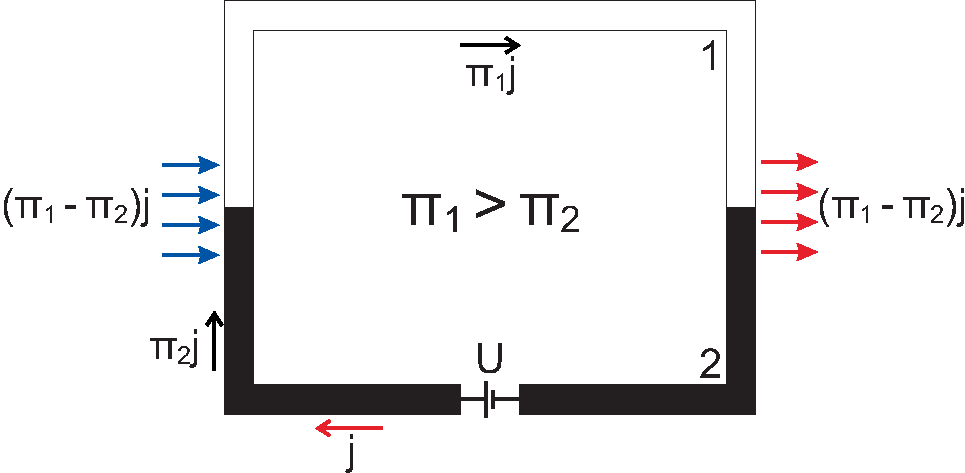
\includegraphics[width=0.8\columnwidth]{Grafiken/Peltiereffekt}
\end{center}

\subsubsection{Supraleitung}
$H_C(T)$: kritische Feldstärke, $I_C$: Kritischer Strom\\
$r$: Radius des Leiters, $T_C$: kritische Temperatur\\
$\Lambda_L$: Londonsche Eindringtiefe, $\mu_0$: absolute Permeabilität
\begin{equation*}
\begin{split}
H_C(T)&=H_{C,0K}\left[1-\left(\frac{T}{T_C}\right)^2\right];\;\;\;\;[H]=\frac{A}{m}\\
I_C&=2\pi rH_C\\
\Lambda_L&=\sqrt{\frac{\lambda_L}{\mu_0}}=\sqrt{\frac{m}{\mu_0n_se^2}}\\
\lambda_L&=\frac{m}{n_se^2}
\end{split}
\end{equation*}

\section{Halbleiter}
\begin{center}
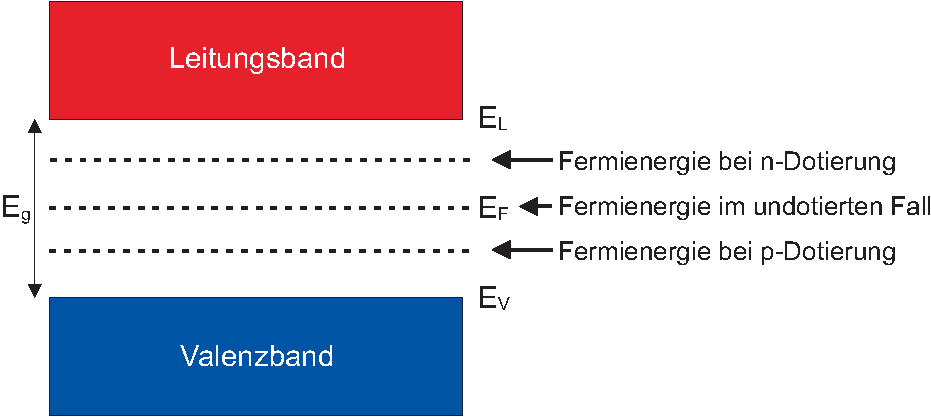
\includegraphics[width=0.95\columnwidth]{Grafiken/Halbleiter_Band}
\end{center}
$f_i(E,T)$: Besetzungswahrscheinlichkeit, $p$: Löcherdichte\\
$n$: Elektronendichte, $D_i(E)$: Zustandsdichte\\
$N_L^*,N_V^*$: effektive Zustandsdichte, $M_L$: Anzahl der äquivalenten Leitungsbandminima in der Brillouinzone\\\\
Wenn ein Element beim Dotieren (je nach Einbau) sowohl als Donator, als auch als Akzeptor wirken kann, so spricht man von einem \textbf{amphoteren Charakter}.
\subsection{Leitungsband}
\begin{equation*}
\begin{split}
f_n(E,T)&=f(E,T)\\
n&=\int\limits_{E_L}^{\infty}D_L(E)f(E,T)dE\\
D_L(E)&=M_L\frac{(2m_n^*)^{\frac{3}{2}}}{2\pi^2\hbar^3}\sqrt{E-E_L};\;\;\;\;E>E_L\\
N_L^*&=2M_L\left[\frac{m_n^*k_BT}{2\pi\hbar^2}\right]^{\frac{3}{2}}\;\;\;\;(M_L\text{ ist meist }1)\\
n&=N_L^*e^{-\frac{E_L-E_F}{k_BT}}\;\;\;\;(\text{Boltzmann-Näherung})\\
\Rightarrow E_L-E_F&=k_BT\cdot ln\left(\frac{N_L^*}{n}\right)
\end{split}
\end{equation*}

\subsection{Valenzband}
\begin{equation*}
\begin{split}
f_p(E,T)&=1-f(E,T)\\
p&=\int\limits_{-\infty}^{E_V}D_V(E)[1-f(E,T)]dE\\
D_V(E)&=\frac{(2m_p^*)^{\frac{3}{2}}}{2\pi^2\hbar^3}\sqrt{E_V-E};\;\;\;\;E<E_V\\
N_V^*&=2\left[\frac{m_p^*k_BT}{2\pi\hbar^2}\right]^{\frac{3}{2}}\\
p&=N_V^*e^{-\frac{E_F-E_V}{k_BT}}\;\;\;\;(\text{Boltzmann-Näherung})\\
\Rightarrow E_F-E_V&=k_BT\cdot ln\left(\frac{N_V^*}{p}\right)
\end{split}
\end{equation*}\\\\
$n_i$: intr. Elektronendichte, $p_i$: intr. Löcherdichte\\
$N_A^-$: Akzeptoren-Dichte, $N_D^+$: Donatoren-Dichte\\
$m_e^*$: effektive Elektronenmasse, $E_F$: Fermienergie\\
\begin{equation*}
\begin{split}
m_e^*&=\left(m_\parallel^*\cdot{m_\perp^*}^2\right)^{\frac{1}{3}}=\left(m_{el}^*\cdot{m_{et}^*}^2\right)^{\frac{1}{3}}\\
m_p^*&=m_h^*=\left({m_{hl}^*}^{\frac{3}{2}}+{m_{hh}^*}^{\frac{3}{2}}\right)^{\frac{2}{3}}\\
n_i&=p_i=\sqrt{N_L^*N_V^*}e^{-\frac{E_g}{2k_BT}}\\
T^{\frac{3}{2}}&\sim \sqrt{N_L^*N_V^*}\\
T^{\frac{3}{2}}&\sim N_L^*,N_V^*\\
E_F&=\frac{E_V+E_L}{2}+\frac{k_BT}{2}ln\left(\frac{N_V^*}{N_L^*}\right)\\
np&=n_ip_i=n_i^2=p_i^2\;\;\;\;\text{(im thermodyn. Gleichgewicht)}\\
n+N_A^-&=p+N_D^+
\end{split}
\end{equation*}
Im Falle einer vollständigen Ionisation gilt:
\begin{equation*}
\begin{split}
\text{bei n-Dotierung}\;\;\;\;N_A^-&=0;\;\;p<<N_D^+\Rightarrow n\approx N_D^+\\
\text{bei p-Dotierung}\;\;\;\;N_D^+&=0;\;\;n<<N_A^-\Rightarrow p\approx N_A^-
\end{split}
\end{equation*}
\subsection{Diffusion}
$L_{n,p}$: Diffusionslänge, $\tau$: Streuzeit, $e$: Elementarladung\\
$\mu_{n,p}$: Beweglichkeit, $D_{n,p}$: Diffusionskonstante\\
$m_p^*$: effektive Lochmasse, $L_D$: Debye-Länge, $\epsilon$: Permittivität\\
$N_D$: Donatoren-Dichte, $n$: Elektronendichte
\begin{equation*}
\begin{split}
L_{n,p}&=\sqrt{D_{n,p}\tau_{n,p}}=\sqrt{\frac{k_BT\mu_{n,p}\tau_{n,p}}{e}}\\
L_D&=\sqrt{\frac{k_BT\epsilon}{e^2N_D}};\;\;\;\;N_D=n\\
D_{n,p}&=\frac{k_BT\mu_{n,p}}{e}\\
\end{split}
\end{equation*}

\subsection{Ausgleich der Minoritätsladungsträger}
$\rightarrow$ S. 129\\\\
$R$: Rekombinationsrate, $r$: Rekombinationsrate\\
$G_L$: optische Generation, $G_T$: thermische Generation
\begin{equation*}
\begin{split}
\frac{dp}{dt}&=\frac{dn}{dt}=G_L+G_T-R=G_L+n_i^2r-npr\\
G_T&=n_i^2r\\
R&=npr\\
\frac{dn}{dt}&\sollsein 0 \Leftrightarrow\text{ stationärer Zustand}
\end{split}
\end{equation*}

\subsection{Ladungstransporteigenschaften}
$\overrightarrow{j}$: Gesamtstromdichte, $\overrightarrow{v}$: Driftgeschwindigkeit\\
$\tau$: Steuzeit, $\sigma$ intrinsische Leitfähigkeit\\
$n,p$: Ladungsträgerdichten, $\mu$: Ladungsträgerbeweglichkeit
\begin{equation*}
\begin{split}
\overrightarrow{j}&=\sigma\overrightarrow{E}=-ne\overrightarrow{v}_n+pe\overrightarrow{v}_p\\
\sigma &=\mu_nen+\mu_pep=e^2\tau\frac{n}{m^*};\;\;\;\;[\sigma]=\frac{S}{m}\\
\mu &=\frac{e\tau}{m^*};\;\;\;\;[\mu]=\frac{cm^2}{Vs}\\
\overrightarrow{v}&=\pm \mu\overrightarrow{E}\;\;\;\;(\text{VZ: }_{\text{Elektronen}}^{\text{Löcher}})
\end{split}
\end{equation*}
\underline{Typische Werte:}
\begin{equation*}
\begin{split}
\text{Metalle: }\sigma&\approx 10^6\frac{S}{m}\\
\text{Halbleiter: }\sigma&\approx 10^{-1}-10^{-6}\frac{S}{m}\\
\text{Isolator: }\sigma&<10^{-7}\frac{S}{m}
\end{split}
\end{equation*}

\section{Dielektrische Eigenschaften von Festkörpern}

\subsection{Polarisation}
$\overrightarrow{P}$: Polarisation, $\overrightarrow{p}$: Dipolmoment, $N$: Teilchendichte\\
$\epsilon_0$: el. Feldkonstante, $\alpha$: Polarisierbarkeit des Atoms\\
$\overrightarrow{E}_a$: primäres äußeres el. Feld, $\epsilon_r$: relative Permittivität\\
$\mathcal{X}$: Suszeptibilität
\begin{equation*}
\begin{split}
\overrightarrow{P}&=N\overrightarrow{p}=N\epsilon_0\alpha\overrightarrow{E}_a;\;\;\;\;[P]=\frac{As}{m^2}\\
\epsilon_r&=1+\mathcal{X}\\
\frac{\alpha N}{3}&=\frac{\epsilon_r-1}{\epsilon_r+2}\;\;\;\;\text{(Claudius-Mosotti-Gleichung)}\\
\Rightarrow \epsilon_r&=\frac{3+2\alpha N}{3-\alpha N}=1+\frac{\alpha N}{1-\underbrace{\frac{\alpha N}{3}}_{\text{Lorentz-Feld}}}\\
\Rightarrow N&=\frac{3(\epsilon_r-1)}{\alpha(\epsilon_r+2)}\\
\alpha N&=\sum\limits_{\forall i}\alpha_iN_i\;\;\;\;\text{(für Moleküle)}
\end{split}
\end{equation*}
Das Lorentz-Feld kann oftmals vernachlässigt werden.

\subsubsection{Elektronische Polarisation}
Elektronenhülle verschiebt sich aufgrund eines anliegenden elektrischen Feldes.\\
$\rightarrow$ induziertes Dipolmoment.\\
Diese Art der Polarisation tritt immer auf und ist temperatur\textbf{un}abhängig.\\\\
$R$: Atomradius, $|\overrightarrow{F}_1|$: auslenkende Kraft, $Z$: Ordnungzahl\\
$|\overrightarrow{F}_2|$: Coulombkraft der inneren Kugelschale\\
$x_0$: Auslenkung der Elektronenhülle / des Kerns\\
$e$: Elementarladung
\begin{equation*}
\begin{split}
\overrightarrow{p}&=\epsilon_0\alpha\overrightarrow{E}_a=4\pi\epsilon_0 R^3\overrightarrow{E}_a\\
\alpha &=4\pi R^3;\;\;\;\;[\alpha]=m^3\\
|\overrightarrow{F}_1|&=Ze|\overrightarrow{E}_a|\\
|\overrightarrow{F}_2|&=\frac{Z^2e^2x_0}{4\pi\epsilon_0 R^3}
\end{split}
\end{equation*}

\subsubsection{Ionische Polarisation}
Positive und negative Ionen werden durch ein äußeres el. Feld gegeneinander verschoben (bei Gitterstruktur).\\
$\rightarrow$ Dipolmoment (temperatur\textbf{un}abhängig)\\\\
$\Delta \overrightarrow{r}$: zusätzlicher Ionen-Abstand durch Verschiebung\\
$q$: Ladung, $\overrightarrow{F}_R$: Rückstellkraft, $\overrightarrow{F}_{el}$: elektrostatische Kraft\\
$U$: potentielle Energie
\begin{equation*}
\begin{split}
\overrightarrow{p}&=\Delta\overrightarrow{r}q\\
\overrightarrow{F}_R&=-\overrightarrow{F}_{el}\\
\left.\frac{\partial U(r)}{\partial r}\right|_{r=r_0}&=0\\
\overrightarrow{F_R}&=-grad(U(r))=-\frac{\partial U(r)}{\partial r}\\
F_R(r_0)&=0\\
F_R(r_0+\Delta r)&=F_R(r_0)+\left.\frac{\partial F_R}{\partial r}\right|_{r=r_0}\cdot\Delta r+...\\
&=-qE\Leftrightarrow \Delta r=-\frac{qE}{\left.\frac{\partial F_R}{\partial r}\right|_{r=r_0}}
\end{split}
\end{equation*}

\subsubsection{Orientierungspolarisation}
Permanente Dipole richten sich im äußeren elektrischen Feld (teilweise) aus (temperaturabhängig).\\\\
$\Theta$: Winkel zwischen $\overrightarrow{E}$ und $\overrightarrow{p}$, $T$: Temperatur\\
$W$: Wahrscheinlichkeit, einen Dipol mit der Energie $U$ bei der Temperatur $T$ zu finden.\\
$k_B$: Boltzmannkonstante, $U$: Energie von Dipol\\
$L(\nu)$: Langevin-Funktion
\begin{equation*}
\begin{split}
\overrightarrow{P}&=N\overrightarrow{p}\overline{cos(\Theta)}\\
P&\sim \frac{1}{T}\\
W(\Theta)&= e^{-\frac{U(\Theta)}{k_BT}}\\
U(\Theta)&=-\overrightarrow{p}\overrightarrow{E}=-p|\overrightarrow{E}|cos(\Theta)\\
L(\nu)&=\overline{cos(\Theta)}=\frac{\overline{W(\Theta)cos(\Theta)}}{\overline{W(\Theta)}}=coth(\nu)-\frac{1}{\nu}\text{ mit }\nu=\frac{p|\overrightarrow{E}|}{k_BT}\\
\nu &>>1:coth(\nu)\rightarrow 1\Rightarrow L(\nu)=1\\
\nu &<<1: coth(\nu)\approx\frac{1}{\nu}+\frac{\nu}{3}\Rightarrow L(\nu)=\frac{\nu}{3}
\end{split}
\end{equation*}

\subsection{Dielektrizitätskonstante}
$\epsilon_r$: komplexe relative Permittivität, $\omega$: Kreisfrequenz\\
$\tau$: Relaxationszeit, $\sigma_{\text{Rest}}$: Restleitfähigkeit
\begin{equation*}
\begin{split}
\epsilon_r&=\epsilon(0)\text{ im statischen Fall}\\
\epsilon_r&=\epsilon'-j\epsilon''=|\epsilon_r|e^{-j\delta}\\
\epsilon'&=\epsilon_{\infty}+\frac{\epsilon_{stat}-\epsilon_{\infty}}{1+\omega^2\tau^2}\\
\epsilon''&=\frac{\epsilon_{stat}-\epsilon_{\infty}}{1+\omega^2\tau^2}\omega\tau\\
\epsilon_{stat}&=\epsilon'(0)>\epsilon_{\infty}\\
\epsilon_{\infty}&=\epsilon(\omega\approx 2\pi\cdot 10^{10}Hz)\\
tan(\delta)&=\frac{\epsilon''}{\epsilon'}=\frac{(\epsilon_{stat}-\epsilon_{\infty})\omega\tau}{\omega^2\tau^2\epsilon_{\infty}+\epsilon_{stat}}\;\;\;\text{(Verlustfaktor)}\\
\sigma_{\text{Rest}}&=\epsilon_0\epsilon''\omega
\end{split}
\end{equation*}
Für das Maximum von $tan(\delta)$ gilt:
\begin{equation*}
\begin{split}
\tau &=\frac{1}{\omega}\sqrt{\frac{\epsilon_{stat}}{\epsilon_{\infty}}}\\
tan(\delta)_{max}&=\frac{\epsilon_{stat}-\epsilon_{\infty}}{2\sqrt{\epsilon_{stat}\epsilon_{\infty}}}\\
\Rightarrow\epsilon_{\infty}&=\epsilon_{stat}\left[1+2tan(\delta)_{max}^2-\sqrt{(1+2tan(\delta)_{max}^2)^2-1}\right]
\end{split}
\end{equation*}
\begin{center}
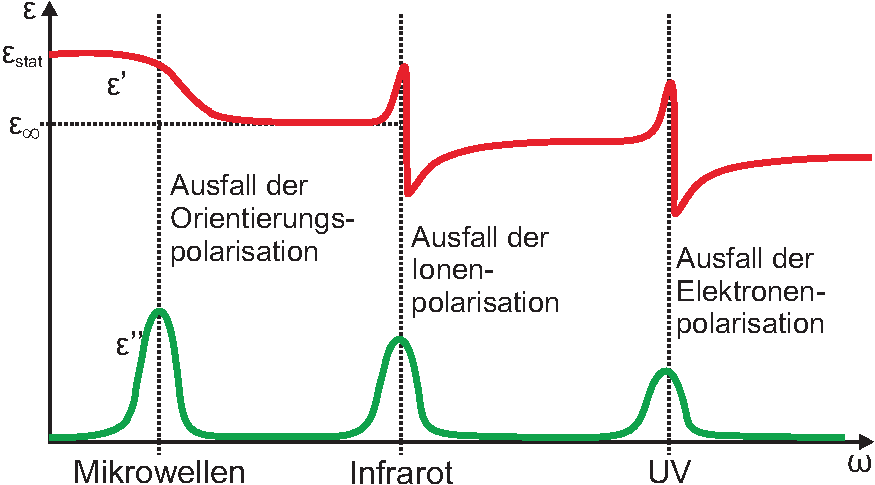
\includegraphics[width=0.9\columnwidth]{Grafiken/Dielektrizitaetskonstante}
\end{center}

\section{Magnetische Eigenschaften von Festkörpern}
$\mu_r$: relative Permeabilität, $\mathcal{X}$: magnetische Suszeptibilität\\
$J$: magnetische Polarisation, $\overrightarrow{H}$: magnetische Feldstärke\\
$M$: Magnetisierung
\begin{equation*}
\begin{split}
\mathcal{X}^m&=\mu_r-1=\frac{J}{\mu_0H}=\frac{M}{H};\;\;\;\;[H]=[M]=\frac{A}{m}\\
\mathcal{X}^m&<0\text{ bzw. }\mu_r<1\Rightarrow\text{ Diamagnetismus}\\
\mathcal{X}^m&>0\text{ bzw. }\mu_r>1\Rightarrow\text{ Paramagnetismus}\\
\mathcal{X}^m&>>0\text{ bzw. }\mu_r>>1\Rightarrow\text{ Ferromagnetismus}
\end{split}
\end{equation*}

\subsection{Elementare magnetische Dipolmomente}
$g$: gyromagn. Verhältnis, $S$: Gesamtspin\\
$J$: Gesamtdrehimpuls, $L$: magnetische Quantenzahl
\begin{equation*}
\begin{split}
g&=1+\frac{J(J+1)+S(S+1)-L(L+1)}{2J(J+1)}\\
1&\leq g\leq 2\\
S&=0\rightarrow g=1\\
L&=0\rightarrow g=2
\end{split}
\end{equation*}

\subsection{Diamagnetismus}
= Auftreten eines zusätzlichen magnetischen Momentes der Elektronenhülle von Atomen unter dem Einfluss eines äußeren Magnetfeldes.\\
Der Diamagnetismus ist temperatur\textbf{un}abhängig und tritt immer auf, wird allerdings vom Para- und Ferromagnetismus überlagert.\\\\
$\overrightarrow{m}$: magnetisches Moment, $N$: Atomdichte\\
$\overline{r^2}$: Erwartungswert des effektiven Bahnradius\\
$Z^*$: effektive Kernladungszahl (Anzahl der Elektronen auf der äußersten Schale abzüglich der Leitungselektronen)
\begin{equation*}
\mathcal{X}_{dia}^m=\frac{\overrightarrow{M}}{\overrightarrow{H}}=\frac{N\overrightarrow{m}}{\overrightarrow{H}}=-\frac{NZ^*e^2\overline{r^2}\mu_0}{6m_0}\\
\end{equation*}

\subsection{Paramagnetismus}
Ist temperaturabhängig und tritt bei Molekülen bzw. Atomen mit magnetischem Dipolmoment auf, d.h. wenn die Elektronenschalen nicht abgeschlossen sind.\\\\
$\mu_B$: Bohrsches Magneton, $k_B$: Boltzmannkonstante\\
$M_{para}$: paramagn. Magnetisierung, $C$: Curie-Konstante
\begin{equation*}
\begin{split}
C&=\frac{Ng^2J(J+1)\mu_B^2\mu_0}{3k_B}\\
\mathcal{X}_{para}^m&=\frac{C}{T}\\
M_{para}&=\mathcal{X}_{para}^mH
\end{split}
\end{equation*}

\subsection{Ferromagnetismus}
Ferromagnetismus tritt nur bis zur Curie-Temperatur auf (danach Paramagnetismus).\\\\
$\Theta$: Curie-Temperatur, $T$: Temperatur
\begin{equation*}
\mathcal{X}^m=\frac{C}{T-\Theta}
\end{equation*}
Oberhalb der Curie-Temperatur tragen folgende Dinge zur magnetischen Suszeptibilität bei:
\begin{enumerate}[label=$\bullet$]
\item Diamagnetismus der Atomhüllen
\item Beitrag der Leitungselektronen (netto paramagnetisch)
\item Paramagnetismus der Atomrümpfe
\end{enumerate}
Der dominante Beitrag ist i.A. der Paramagnetismus.

\subsection{Leitungselektronen}
$n$: Elektronendichte, $T_F$: Fermitemperatur
\begin{equation*}
\begin{split}
\mathcal{X}_{para}^m&=\frac{3n\mu_0\mu_B^2}{2k_BT_F}\\
\mathcal{X}_{dia}^m&=-\frac{1}{3}\mathcal{X}_{para}^m\\
\mathcal{X}^m&=\mathcal{X}_{para}^m+\mathcal{X}_{dia}^m=\frac{n\mu_B^2\mu_0}{k_BT_F}
\end{split}
\end{equation*}

\section{Physikalische Konstanten}
\begin{tabular}{ll}
Atomare Masseneinheit & $u=1,66\cdot 10^{-27}kg$\\\\
Avogadro-Konstante & $N_A=6,022\cdot 10^{23}\frac{1}{mol}$\\\\
Elektrische Feldkonstante & $\epsilon_0=8,85\cdot 10^{-12}\frac{F}{m}$\\\\
Elektron Ruhemasse & $m_e=9,109\cdot 10^{-31}kg$\\\\
Elementarladung & $e=1,602\cdot 10^{-19}C$\\\\
Magnetische Feldkonstante & $\mu_0=4\pi\cdot 10^{-7}\frac{Vs}{Am}$\\\\
Bohrsches Magneton & $\mu_B=\frac{e\hbar}{2m_0}=9,27\cdot 10^{-24}Am^2$\\\\
Plancksches Wirkungsquantum & $h=6,626\cdot 10^{-34}Js$\\\\
Rydberg-Konstante & $R_\infty=1,0974\cdot 10^7\frac{1}{m}$\\\\
Rydberg-Konstante & $R_H=1,0968\cdot 10^7\frac{1}{m}$\\\\
Boltzmannkonstante & $k_B=1,38\cdot 10^{-23}\frac{J}{K}$\\\\
Gaskonstante & $R=8,31\frac{J}{Kmol}$
\end{tabular}
\\\\\\\\\\
Lizenz: CC BY-NC-SA 3.0\\
\url{http://creativecommons.org/licenses/by-nc-sa/3.0/de/}

\end{document}








